\chapter{Design \& Implementation}
\label{chapter:design}

\section{NCS Software}

The NCS simulator provides the ability to simulate biologically-realistic neural interactions at a large scale. While NCS performs the core goals of a brain simulator, there is a much larger set of functionality that is needed for a simulator than running the simulation itself. This functionality includes building the simulation, running the simulation, storing simulation data, and analyzing results, which is imperative to the researcher using any brain simulator. We designed a suite of tools that surround the NCS simulator that provide users the ability to perform these tasks. These tools include a consistent storage and management system for the simulations users create, a programmatic Python interface, a web-based interface for building, running and analyzing simulations, and a way to visualize the results of the simulation. With the construction of these tools we have also introduced a new architectural concept, the client-server model, that is unique to current brain simulators. A diagram showing a high-level overview of NCS and its surrounding software can be found in Figure \ref{fig:ncs_architecture}

\begin{figure}
\begin{center}
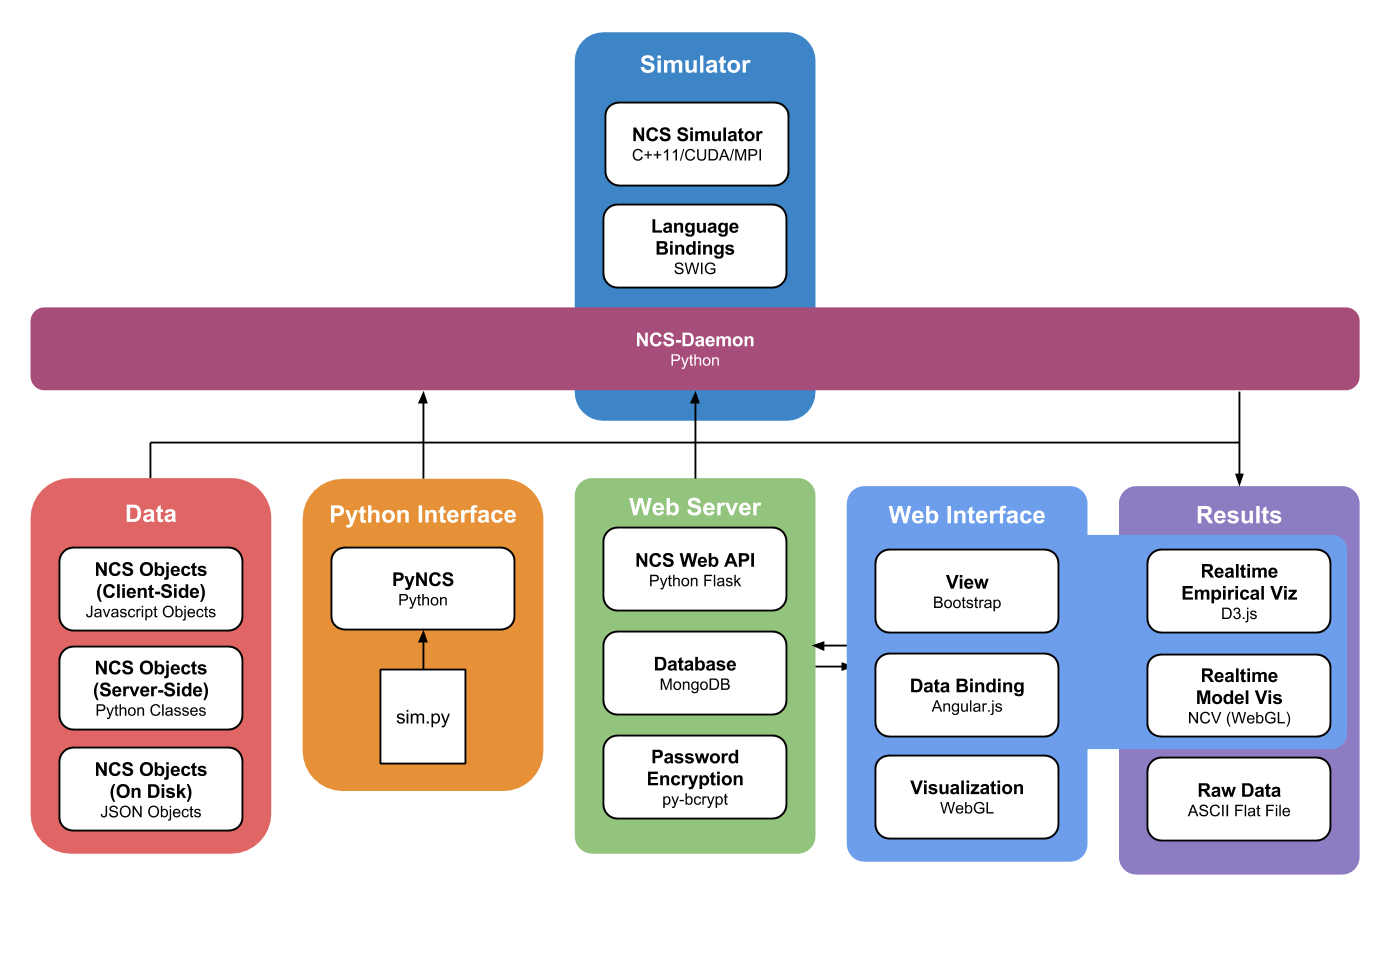
\includegraphics[height=\textheight,width=6in,keepaspectratio]{figures/ncs_architecture.png}
\caption[NCS Architecture]{This diagram is a graphical representation of the NCS software suite. The simulator performs the core simulation tasks and is shown in dark blue. NCS-Daemon acts as a intermediary between external services and the simulator and provides a single point of entry for all simulator tasks. It allows NCS to focus on being as fast as possible by handling the organizational outside the simulator codebase. The tools that surround the simulator include a Python interface, and a web interface. These services interact with NCS-Daemon to gain access to the simulator.\label{fig:ncs_architecture}}
\end{center}
\end{figure}

\section{NCS-Daemon}

Part of the goal in designing NCS was to provide the simulator as a service that multiple clients could interact with rather than as a program that is run from the command line. To do this, a process or daemon must be consistently running on the root node of the NCS cluster that accepts connections from clients attempting to use the simulator. Additionally, a method of transport is needed to carry information to the daemon from the clients and vice versa. As discussed earlier, one of the best methods to transfer textual data over a network is the HTTP protocol. HTTP is ubiquitous and libraries exist for using it in virtually every programming language, making it an easy choice for implementing the communication fabric between the daemon and the clients. Finally, HTTP is a client-server-based protocol, which suits the goal of the project perfectly.

There are a myriad of different libraries and frameworks to choose from to create a server using HTTP as the underlying protocol. Since the low-level simulator functions are exposed using a thin Python layer, it makes sense to choose a Python-based HTTP library to handle the connections to the simulator. Several popular libraries exist as Python modules: the most popular of which is Django\cite{googletrends2014django}. Django is a so-called full-stack web application framework, as it has facilities for creating database entities, an administrative interface, form-validation, and many other features that make it advantageous to use as a general web application framework. NCS-Daemon, however, would not make use of the vast majority of these features, making Django superfluous for the requirements of the application. Another web framework called Flask\cite{grinberg2014flask} provides a more minimal set of functionality. It provides the ability to designate \emph{routes} that call certain Python functions when a request comes in to a certain URI, making it very easy to implement a REST interface. Flask also has a host of extensions that help extend the functionality of the application including WebSockets and integration with MongoDB, a popular JSON-based NoSQL database. Because of its simplicity and extensibility, we chose to implement the daemon using the Flask web application framework. A simple "Hello, world" Flask application can be found in Figure \ref{fig:flask_hello_world}.

\begin{figure}
\begin{center}
\begin{lstlisting}[language=Python]
from flask import Flask
app = Flask(__name__)

@app.route("/")
def hello():
    return "Hello World!"

if __name__ == "__main__":
    app.run("localhost", 8000)
\end{lstlisting}
\caption[Flask Hello World]{This Flask application serves the plain text "Hello World" when an HTTP client sends a GET request to the '/' route.\label{fig:flask_hello_world}}
\end{center}
\end{figure}

To design NCS-Daemon as a RESTful service, a number of resources needed to be defined. The first resource is the \emph{simulator} resource. The \emph{simulator} resource refers to the current status of the simulator. A GET request to this resource will provide information on the status of the simulator, a POST request containing simulation data will attempt to start a new simulation, and a DELETE request will attempt to stop the currently running simulation. The next resource is the \emph{simulation} resource. The simulation resource refers to a specific simulation created by a user. This resource allows the GET and DELETE methods. The GET method returns information about the simulation specified, including log information, reports related to the sim, and the simulation object that was run by the simulator. A DELETE request to a specified simulation resource will delete that simulation, as well as any data associated with it. The next resource is the \emph{report} resource. The \emph{report} resource requests the contents of a report generated by a previous simulation. It accepts the GET and DELETE methods, which instruct the server to provide the report, and remove the report from disk respectively. In the event a report was specified as a streaming report meant for WebSockets, the resource will return an error. The final resource is the \emph{login} resource. This resource provides an endpoint for users to authenticate with the server which is an important component of NCS-Daemon.

When implementing any network-based application, security is always a matter of concern, especially when the application is facing the Internet. Preventing unauthorized use of the NCS simulator and protecting user information are the main problems with regard to application security. To prevent unauthorized use of the simulator a login system was created. To use the simulator, the user must have an account on the server. Next, before any interaction with the daemon, the user must first send a POST request to the \emph{/login} route on the server, supplying their username and password. In response, the server sends an authorization token specific to that user. Each request to the server must contain this authorization token in the HTTP headers or the server will reject the request as unauthorized. By providing the token to users, it prevents their credentials from being passed with each request. If an attacker were to begin intercepting communications between the client and server after the user has logged in, he would only gain the access token. The attacker would still be able to gain access to the simulator for a certain time, but the user's credentials would remain secret and could not be used to gain access to external accounts such as email and bank accounts registered using the same password. To completely protect access to the simulator and the users credentials, the connection to the server must be made over HTTPS using SSL or TLS, which are used to create a completely secure connection that cannot be decoded by other parties during or after transmission.

NCS-Daemon is implemented as a RESTful interface and as such exposes these resources to clients in the form of routes. In addition to the traditional RESTful routes exposed by the application, NCS-Daemon also has two different WebSocket routes that are also available for streaming live data to the client provided the client has a library to interact with the WebSocket protocol. The routes exposed by NCS-Daemon as well as their descriptions and allowed methods can be found in Table \ref{table:routes}.

\begin{table}
\def\arraystretch{1.5}
\begin{tabular}{ l | p{0.75in} | p{3.2in} }
Route & Methods & Resource Description \\
\hline
/login & POST & The login route accepts requests containing a username and password and responds with an access token provided the credentials were correct.  \\
\hline
/simulator & GET POST DELETE & The simulator route provides a resource for the state of the simulator. A GET request returns information about the current status of the simulator. A POST request will instruct the daemon to start a simulation. Finally, a DELETE request instructs the daemon to cancel the current simulation.  \\
\hline
/simulation/:id & GET DELETE & The simulation route provides a resource for past simulations. A GET request returns information about the simulation requested. A DELETE request instructs the daemon delete the specified simulation.  \\
\hline
/report/:id & GET & The report route provides the report generated by a simulation, including whether it can be streamed through a WebSocket.  \\
\hline
/report\_stream/:id & WebSocket & The report\_stream route is used for streaming live report data over a WebSocket interface.  \\
\hline
/geometry\_stream & WebSocket & The geometry\_stream WebSocket can be used to stream the locations and geometry of neurons and connections for a realtime visualization.  \\
\end{tabular}
\caption[REST Interface Routes and Descriptions]{This table shows the routes, methods and descriptions for NCS-Daemon's RESTful interface.\label{table:routes}\vspace{0.25in}}
\end{table}

NCS-Daemon is designed to be fully testable and is designed with good software engineering practices. The project repository is hosted on GitHub and is integrated with the Travis Continuous Integration service. This service runs the project's tests each time a developer attempts to update the repository and alerts the user when their changes break the tests. Additionally, the service outputs the code coverage of the tests, which measure the amount of code in the repository was run during the tests, which keep track of how effective the testing suite is. Ideally, this number should be as close to 100\% as possible. The software class diagram for NCS-Daemon can be found in Figure \ref{fig:ncs_daemon_diagram} and the GitHub repository showing the NCS-Daemon README with the testing and coverage badges can be found in Figure \ref{fig:readme}.

\begin{figure}
\begin{center}
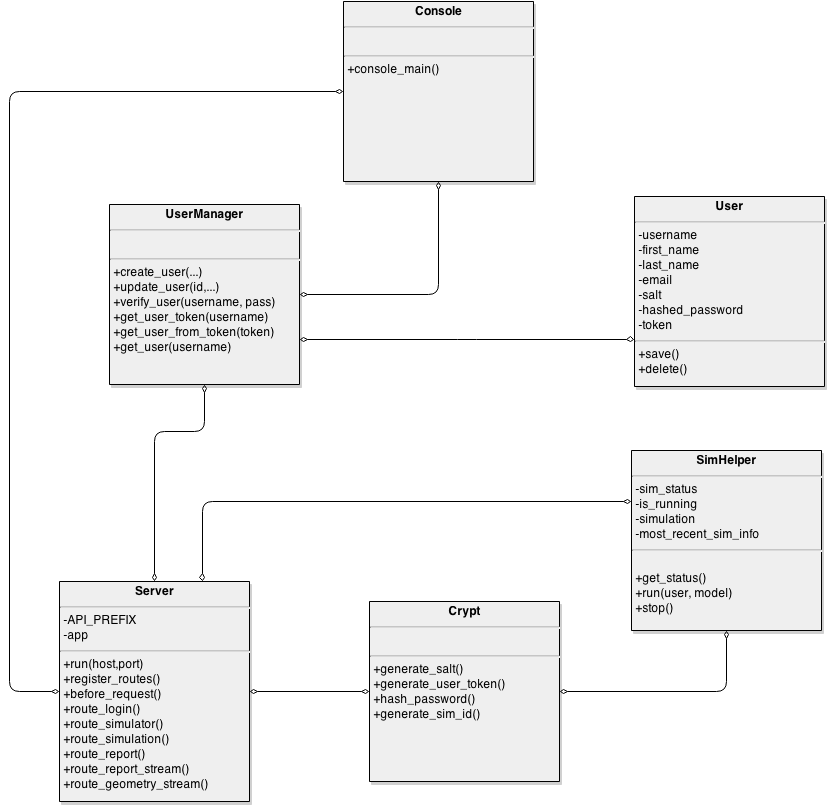
\includegraphics[height=\textheight,width=6in,keepaspectratio]{figures/ncs_daemon_diagram.png}
\caption[NCS-Daemon Class Diagram]{This is the NCS-Daemon's class diagram with testing components omitted.\label{fig:ncs_daemon_diagram}}
\end{center}
\end{figure}

\begin{figure}
\begin{center}
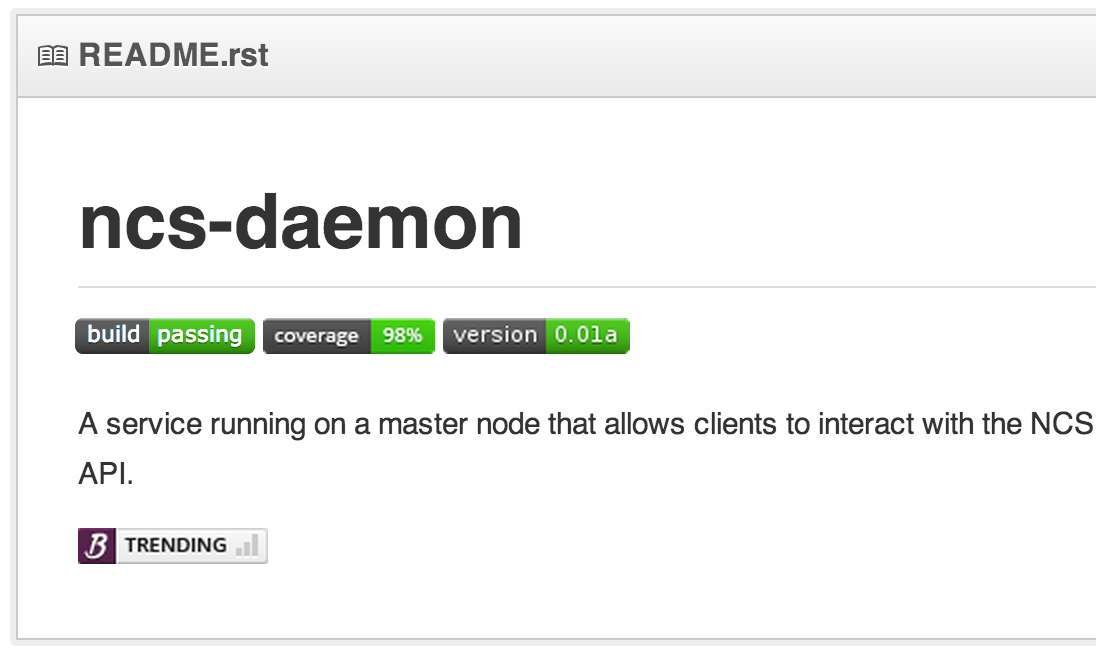
\includegraphics[height=\textheight,width=5in,keepaspectratio]{figures/readme.png}
\caption[NCS-Daemon GitHub README]{The README file for NCS-Daemon contains badges that link to the current testing state of the project, including if its tests are passing, and what the code coverage percentage is.\label{fig:readme}}
\end{center}
\end{figure}

\section{Simulation Concepts \& Transfer Format}

NCS simulations are defined as a hierarchical structure of groups and neuron groups as well as several other entities each with their own parameters. These entities include neurons, synapses, stimuli, reports, neuron\_aliases, and synapse\_aliases. Neuron entities contain the model used to calculate whether or not a neuron will fire on a particular time tick. Neurons can be of several types, each with their own set of parameters that affect the behavior of the neuron. Currently, the simulator supports Leaky-Integrate-and-Fire (LIF), Hodgkin-Huxley, and Izhikevich models for neurons. Synapses define the properties of connections between neurons including synaptic learning and plasticity. Stimuli define where electrical current will be applied during the simulation and how it should be delivered. Reports define which properties and which neurons or synapses should be collected and either streamed over a WebSocket or written to disk during the simulation. Lastly, neuron\_aliases and synapse\_aliases provide a way to refer to large collections of neurons or synapses under a single name instead of all their collective names, reducing the work required for referencing large groups or neurons or synapses.

Since NCS doesn't have native support for higher-level constructs, a system needed to be developed allows for users to organize the groups of cells more effectively. To accomplish this, we created a hierarchical system of groups as a way to structure the model. A group may contain multiple types of entities, the first of which are subgroups. Subgroups are instances of other groups placed within a larger group that have a label that distinguishes themselves from other subgroups in the same group. Groups can also contain neuron groups, which are simply collections of neurons of the same type that act as a single unit. Groups are also where connections are defined. A connection is created between two neuron groups with a synapse type and a certain probability of connection between them. Finally, aliases are created within groups. Aliases allow a single label to refer to multiple objects. For example, if there are two neuron groups labeled "A" and "B", then a neuron alias named "AB" could be created that refers to both of these subgroups. This system allows users to better organize their models, and create larger models more effectively than creating numerous unorganized neuron groups. This system of organization is illustrated in Figure \ref{fig:group_diagram}.

\begin{figure}
\begin{center}
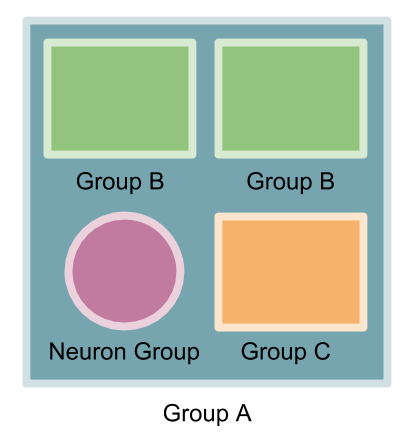
\includegraphics[height=\textheight,width=5in,keepaspectratio]{figures/group_diagram.png}
\caption[Group Hierarchy Diagram]{This diagram shows a visual representation of a group in NCS. Group A contains two instances of Group B, a neuron group, and another group, Group C. A JSON representation of a group can be found in Figure \ref{fig:group_json}.\label{fig:group_diagram}}
\end{center}
\end{figure}

In order to transfer and store simulations, some kind of textual representation for the simulation model and its entities must be created. Due to the hierarchical nature of the simulation model, with simulations possibly containing many of the same group type, the tree of groups could grow at a sizable rate if this structure were fully expanded into JSON. This makes the size of the files much larger, which is bad for both transporting the JSON over a network or storing it on disk. Additionally, it makes decoding the simulation once it reaches the daemon more complicated and slow due to the redundant information and very deep model structure. To combat this, we have implemented a normalized approach to storing the data in a textual format, akin to the concepts of a relational database. Instead of expanding the simulation tree into its full form, the tree is traversed and groups are added to a list of groups. Inside the groups, rather than expanding subgroups into their corresponding JSON, we maintain a reference to the other group in the form of a unique identifier, that is generated randomly. This saves space by reducing redundancy that would be common in many models. Since the other entities are not defined in a hierarchical fashion, they do not need to be normalized and can be added to a list with other entities of the same type. A template showing the simulation transfer format with normalized groups can be found in Figure \ref{fig:empty_transfer_format}.

\begin{figure}
\begin{center}
\begin{lstlisting}
{
    "top_group": "5728ec1d381bad25744bc54c42ba425",
    "neurons": [
    
    ],
    "synapses": [
    
    ],
    "stimuli": [
    
    ],
    "reports": [
    
    ],
    "groups": [
    
    ],
    "neuron_aliases": [
    
    ],
    "synapse_aliases": [
    
    ]
}
\end{lstlisting}
\caption[JSON Transfer Format]{The JSON transfer format without any entities defined. The \emph{top\_group} property specifies the id of the topmost group in the simulation heirarchy. When a client submits a simulation to NCS-Daemon the arrays would be populated with data.\label{fig:empty_transfer_format}}
\end{center}
\end{figure}

In addition to their specifications, entities also contain metadata that describes information about the entity, such as its type, name, description, author, institution, and author's email. When stored on disk or in a database such as MongoDB, this metadata can be used to determine where a model was created, who it was created by, and which scientific papers it might have been created for or from. This will aid researchers in collaborating on experiments, and keeping models organized. An example of an Izhikevich neuron entity including its metadata can be found in Figure \ref{fig:izh_json} and a group entity with subgroups, neuron groups, aliases, connections and metadata can be found in Figure \ref{fig:group_json}.

\begin{figure}
\begin{center}
\begin{lstlisting}
{
    "_id": "c4f5ea85f4c5ae86c4ebc4a854",
    "entity_type": "neuron",
    "entity_name": "neuron_izh_1",
    "description": "This is an extended description of the entity",
    "author": "Nathan Jordan",
    "author_email": "njordan@cse.unr.edu",
    "specification": {
        "type": "izhikevich",
        "a": 0.02,
        "b": 0.2,
        "c": -65.0,
        "d": 8.0,
        "u": -12.0,
        "v": -65.0,
        "threshold": 30
    }
}
\end{lstlisting}
\caption[JSON Izhikevich neuron model]{An Izhikevich neuron model with metadata represented in JSON. The metadata surrounds the Izhikevich parameters contained within the specification object.\label{fig:izh_json}}
\end{center}
\end{figure}

\lstset{
  basicstyle=\tiny\ttfamily
}

\begin{figure}
\begin{center}
\begin{lstlisting}
{
    "_id": "df90sahf0sd9ha8sdhf8dhsa",
    "entity_type": "group",
    "entity_name": "BasalGanglia",
    "description": "This is an extended description of the entity",
    "author": "Nathan Jordan",
    "author_email": "njordan@cse.unr.edu",
    "specification": {
        "geometry": {
            "width": 100.0,
            "height": 200.7,
            "depth": 300.3
        },
        "subgroups": [
            {
                "group": "sdfh8ahsdf80has0d89fh0as9dhf",
                "label": "striatum",
                "location": {"x": 123.5, "y": 456.5, "z": 789.5}
            },
            {
                "group": "hf8as0df8asdhf80ahsd80f",
                "label": "pallidum",
                "location": {"x": 2354.5, "y": 456.5, "z": 543.5 }
            }
        ],
        "neuron_groups": [
            {
                "neuron": "hfd80sahs80dhf0shda90fhshdf",
                "label": "gpe",
                "count": 400,
                "geometry": {"width": 100.4, "height": 200.7, "depth": 300.8},
                "location": {"x": 234.9, "y": 456.4, "z": 543.2}
            },
            {
                "neuron": "hasd890fhas80fhas80dhf",
                "count": 30,
                "label": "gpi",
                "geometry": {"width": 100.1, "height": 200.6, "depth": 300.7},
                "location": {"x": 784.4, "y": 926.1, "z": 999.2}
            }
        ],
        "neuron_aliases": [
            {
                "alias": "gpx",
                "labels": ["gpe", "gpi"],
                "aliases": ["an_alias"]
            }
        ],
        "synaptic_aliases": [
            {
                "alias": "sample_synapse_alias",
                "labels": ["GP_synapse"]
            }
        ],
        "connections": [
                {
                    "presynaptic": "gpe",
                    "postsynaptic": "gpi",
                    "probability": 0.5,
                    "synapse": "hfd8nfiodnsa80dbhfbas80df",
                    "recurrent": false
                }
        ]
    }
}
\end{lstlisting}
\caption[JSON Group Definition]{JSON Group specification with metadata parameters.\label{fig:group_json}}
\end{center}
\end{figure}

\lstset{
  basicstyle=\footnotesize\ttfamily
}


\section{PyNCS}

Now that the server and transfer schema have been defined, there needs to be a convenient way to interact with the server without having to deal with HTTP and the JSON representation during transfer. To address this, we have created a Python library called PyNCS. PyNCS allows users to communicate with an NCS server using an intuitive Python interface. To connect to the server, the user instantiates a \emph{Simulator} object with their username and password. If the library fails to connect to the simulator, an authentication exception is thrown. An example showing the usage of the simulator via PyNCS can be found in Figure \ref{fig:simulator_connection}. Models are created using Python classes that are defined in the PyNCS package. These classes provide a way to create models in an object-oriented fashion without use of dictionaries or less-structured Python types. When creating entity objects, the parameters are checked against a known list of acceptable parameters for that entity as to prevent mistakes when creating a model, and alerting the user to their mistakes before the simulation is run, so they can more easily identify where the error is and fix it quickly. For example, creating an Izhikevich neuron and specifying \emph{x} as a parameter will throw an exception. An example of this functionality can be found in Figure \ref{fig:pyncs_izh}.

\begin{figure}
\begin{center}
\begin{lstlisting}[language=Python]
# Correct
server = Simulator(
    host='ncscluster.example.edu',
    port=8081,
    username='my_username',
    password='my_password'
)

# Throws ConnectionError
server = Simulator(
    host='no_ncsdaemon_here.example.edu',
    port=8081,
    username='my_username',
    password='my_password'
)

# Throws AuthenticationError
server = Simulator(
    host='ncscluster.example.edu',
    port=8081,
    username='my_username',
    password='not_my_password'
)
\end{lstlisting}
\caption[PyNCS Simulator Example]{This example gives three different scenarios for connections. The first example results in a successful connection, the second example attempts to connect to a host where NCS-Daemon is not running, and the last example attempts to connect to NCS-Daemon with the incorrect credentials.\label{fig:simulator_connection}}
\end{center}
\end{figure}

\begin{figure}
\begin{center}
\begin{lstlisting}[language=Python]
# This successfully defines an Izhikevich neuron
izh = IzhNeuron(
    a=0.5,
    b=0.5,
    c=0.5,
    d=8.0,
    u=-12.0,
    v=Normal(-65.0, 0.5),
    threshold=30.0
)

# This throws an EntityError because we tried to specify x
izh = IzhNeuron(
    a=0.5,
    b=0.5,
    c=0.5,
    d=8.0,
    u=-12.0,
    x=10.0,
    threshold=30.0
)
\end{lstlisting}
\caption[PyNCS Izhikevich Model]{This figure shows how an Izhikevich neuron would be declared in PyNCS. The first example successfully creates an Izhikevich neuron type, whereas the second example results in an exception.\label{fig:pyncs_izh}}
\end{center}
\end{figure}

The Python classes also enforce which parameters are required and optional. This allows users to only specify which parameters that are pertinent to the entity they are creating without specifying extra parameters that are empty. This makes PyNCS code more readable by reducing a level of verbosity, makes the code faster to write, and keeps code size to a minimum.

Once the model and other entities have been created, the user must create a \emph{Simulation} object. The simulation object encapsulates a single instance of a simulation. The most important service the \emph{Simulation} object performs is maintaining references to the reports generated by the simulation. These reports can be downloaded to the client from the server for further processing, visualization or anything else the user might wish to use the simulation data for. They are not downloaded automatically due to the possibility that the reports can become quite large dependant on the number of neurons or synapses being reported on and the frequency at which data on these entities is collected. The \emph{Simulation} object can also be used as a WebSocket client to stream realtime data from the server. Lastly, the simulation object contains diagnostic information and log data related to the simulation so the user can view and address any potential problems that may arise during a simulation. The \emph{Simulation} object can only be used for one simulation; to create and run another simulation, an additional \emph{Simulation} object must be create. An example of a \emph{Simulation} object being created and run can be found in Figure \ref{fig:pyncs_run_sim}.

\lstset{
  basicstyle=\tiny\ttfamily
}

\begin{figure}
\begin{center}
\begin{lstlisting}[language=Python]
izh = IzhNeuron(
    a=0.5,
    b=0.5,
    c=0.5,
    d=8.0,
    u=-12.0,
    v=Normal(-65.0, 0.5),
    threshold=30.0
)
syn = FlatSynapse(
    delay=10.0,
    current=60.0
)
nrn_grp1 = NeuronGroup(
    neuron=izh,
    count=30,
    label="izh1",
    geometry=Geometry(),
    location=Location()
)
nrn_grp2 = NeuronGroup(
    neuron=izh,
    count=50,
    label="izh2",
    geometry=Geometry(),
    location=Location(),
)
conn = Connection(
    presynaptic="izh1",
    postsynaptic="izh2",
    probability=0.5,
    synapse=syn
)
grp = Group(
    entity_name="my_group",
    subgroups=[],
    neuron_groups=[nrn_grp1, nrn_grp2],
    neuron_aliases=[],
    synapse_aliases=[],
    connections=[conn]
)
stim = RectCurrentStimulus(
    amplitude=3.0,
    width=2,
    frequency=10,
    probability=0.6,
    time_start=0,
    time_end=1,
    destinations=["my_group:izh1"]
)
rpt = Report(
    report_method=Report.METHOD_FILE,
    report_type=Report.TYPE_NEURON,
    report_target=[nrn_grp1],
    probability=0.5,
    time_start=0.0,
    time_end=1.0
)
sim = Simulation(
    top_group=grp,
    stimuli=[stim],
    reports=[rpt]
)
server = Simulator(
    host='ncscluster.example.edu',
    port=8081,
    username='my_username',
    password='my_password'
)

if server.get_status() == Simulator.IDLE:
    server.run(sim)
\end{lstlisting}
\caption[PyNCS Running Simulation]{This figure shows how a simulation would be created and run in PyNCS. The sim object is created using the top-level model and a list of stimuli and reports. The Simulator object is created using a hostname and port as well as a username and password which establishes a connection to NCS-Daemon. Once a connection has been established, the status of the simulator can be checked. If the simulator is idle, we can run the created simulation.\label{fig:pyncs_run_sim}}
\end{center}
\end{figure}

\lstset{
  basicstyle=\footnotesize\ttfamily
}

\section{Web Interface}

While the PyNCS interface provides a way for users with knowledge of programming (specifically Python programming) to create and run simulations programmatically, this is a skill set that many potential neuroscientists using the NCS simulator may not have or want to exercise. To address the needs of all neuroscientists, a more user-friendly and less-technical interface is needed to interact with the brain simulator. Simulators such as NEURON and GENESIS discussed in the background section use old interfaces developed for native windowing environments like X11. The problem with these interfaces is that they are now antiquated, as newer technologies exist to create these environments for modern operating systems. Additionally, they must be run on the users computer directly, forcing them to install software on their machine which may not be desirable. To address these problems, we have created a web-based interface that acts as a client to the NCS-Daemon server and allows neuroscientists to create simulations using only a web browser.

To create the web interface we took advantage of a couple tools that would greatly reduce design time. Firstly, we used the Bootstrap front-end framework to create a consistent look and feel, and save a lot of development time by not having to develop custom UI widgets. Secondly, we made use of AngularJS as the Javascript framework powering the page. Angular allows easy integration with the DOM without having to directly manipulate it as well as providing a way to easily interact with the RESTful interface of NCS-Daemon. Currently, there are five tabs in the NCS Web Interface: model builder, sim builder, reports, model database, and robot simulator. 

The model builder, shown in Figure \ref{fig:model_builder}, is a graphical way for users to create their models. The design of the model builder posed some particularly difficult UI design challenges. While some entities like neurons are single-layer entities, group entities form a hierarchical structure that could be several layers deep. Users need to be able to navigate efficiently through these levels and do so without feeling like the UI has become too cluttered. We felt that a tree-type interface would lead to too much clutter and greatly degrade user experience. To develop a more effective interface, we took some queues from file explorers of different operating systems. File explorers also work on a hierarchical data set (a filesystem is a tree) and have been developed to make it easy for users to navigate around the filesystem and perform operations on it. A particular example of this is the Windows Explorer interface that uses breadcrumbs to show the user where they are and a main content area where the content of the location is displayed. 

\begin{figure}
\begin{center}
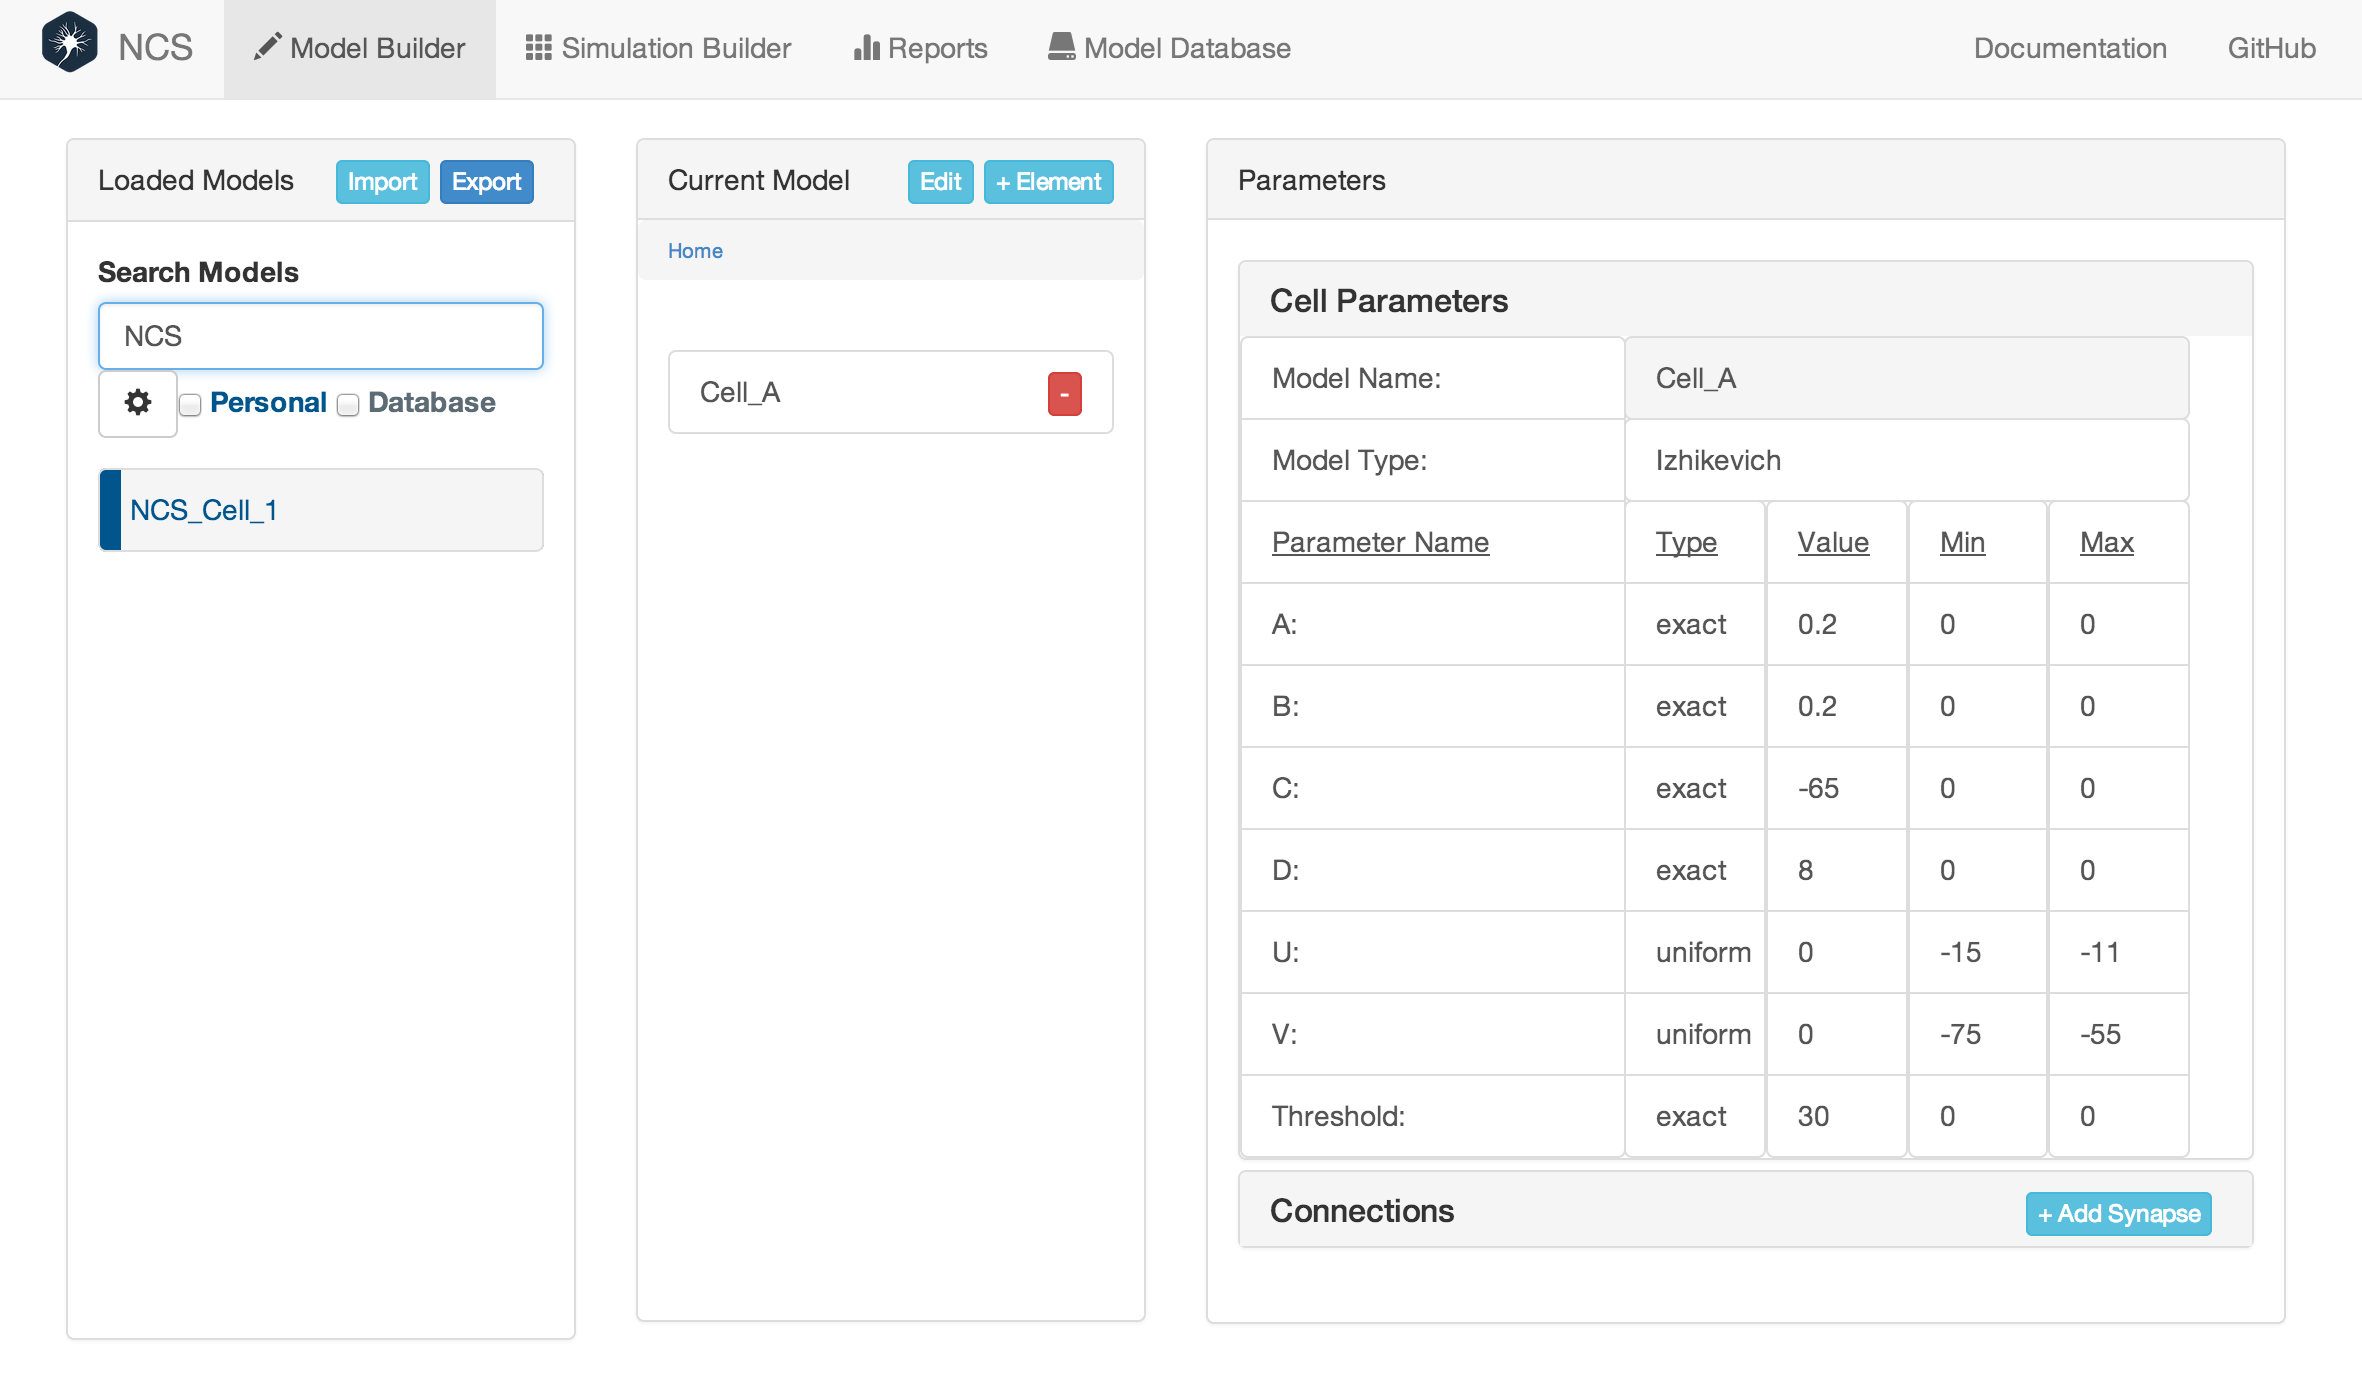
\includegraphics[height=\textheight,width=5in,keepaspectratio]{figures/model_builder.png}
\caption[Model Builder]{The model builder is organized into three sections split vertically across the page. The leftmost panel contains models that the user has built or loaded from a file or database. The second panel displays entities that are within the currently active group. The rightmost panel displays parameters of a selected entity. In this case, it is displaying the Izhikevich parameters for Neuron\_1.\label{fig:model_builder}}
\end{center}
\end{figure}

In our design, we implemented a system in which breadcrumbs are used to navigate the tree and keep track of where the user is in the hierarchy (similar to file explorer) and a content area in the form of a panel updates as the user navigates. As the user moves through the groups they are creating, links are created and removed along a top bar that indicates where they are in the model. If they want to move to a different position in the hierarchy, they simply click the link corresponding to the name of the group they want to move to and the content area updates accordingly. In the content area is a list of subgroups the user can further navigate into. When the user selects one of these subgroups a new subgroup is created, the user is shown the contents of the new subgroup (when created it is empty) and a breadcrumb is added to the list. 

The rightmost panel is where model specifications are created. This panel lets the user modify the properties of entities they have selected. For example, if the user were to select a neuron from the model selection list on the left parameters related to the neuron would be editable to the user on the right panel, such as the voltage threshold or resting potential. Values updated here are propagated to the back-end model and are updated there.

Once the user has created or imported the model they wish to execute in the simulator, they then switch to the sim builder tab. The sim builder tab, shown in Figure \ref{fig:sim_builder} allows the user to create interactions with the model that they have built and actually create the simulation. Firstly, the user should create at least one stimulus to inject into a select group of cells within the model to bring it to life. The stimulus can be generated from a few different sources, including a file-based stimulus, or a socket-based stimulus. The socket-based stimulus provides external programs the ability to provide input to the simulation. Once the stimuli are created, the user can create reports for the model. Reports are the way data can be extracted from the simulation, and several metrics can be reported on, including synaptic plasticity to membrane potential. Once the user is finished with these tasks, the simulation can be run from this tab.

\begin{figure}
\begin{center}
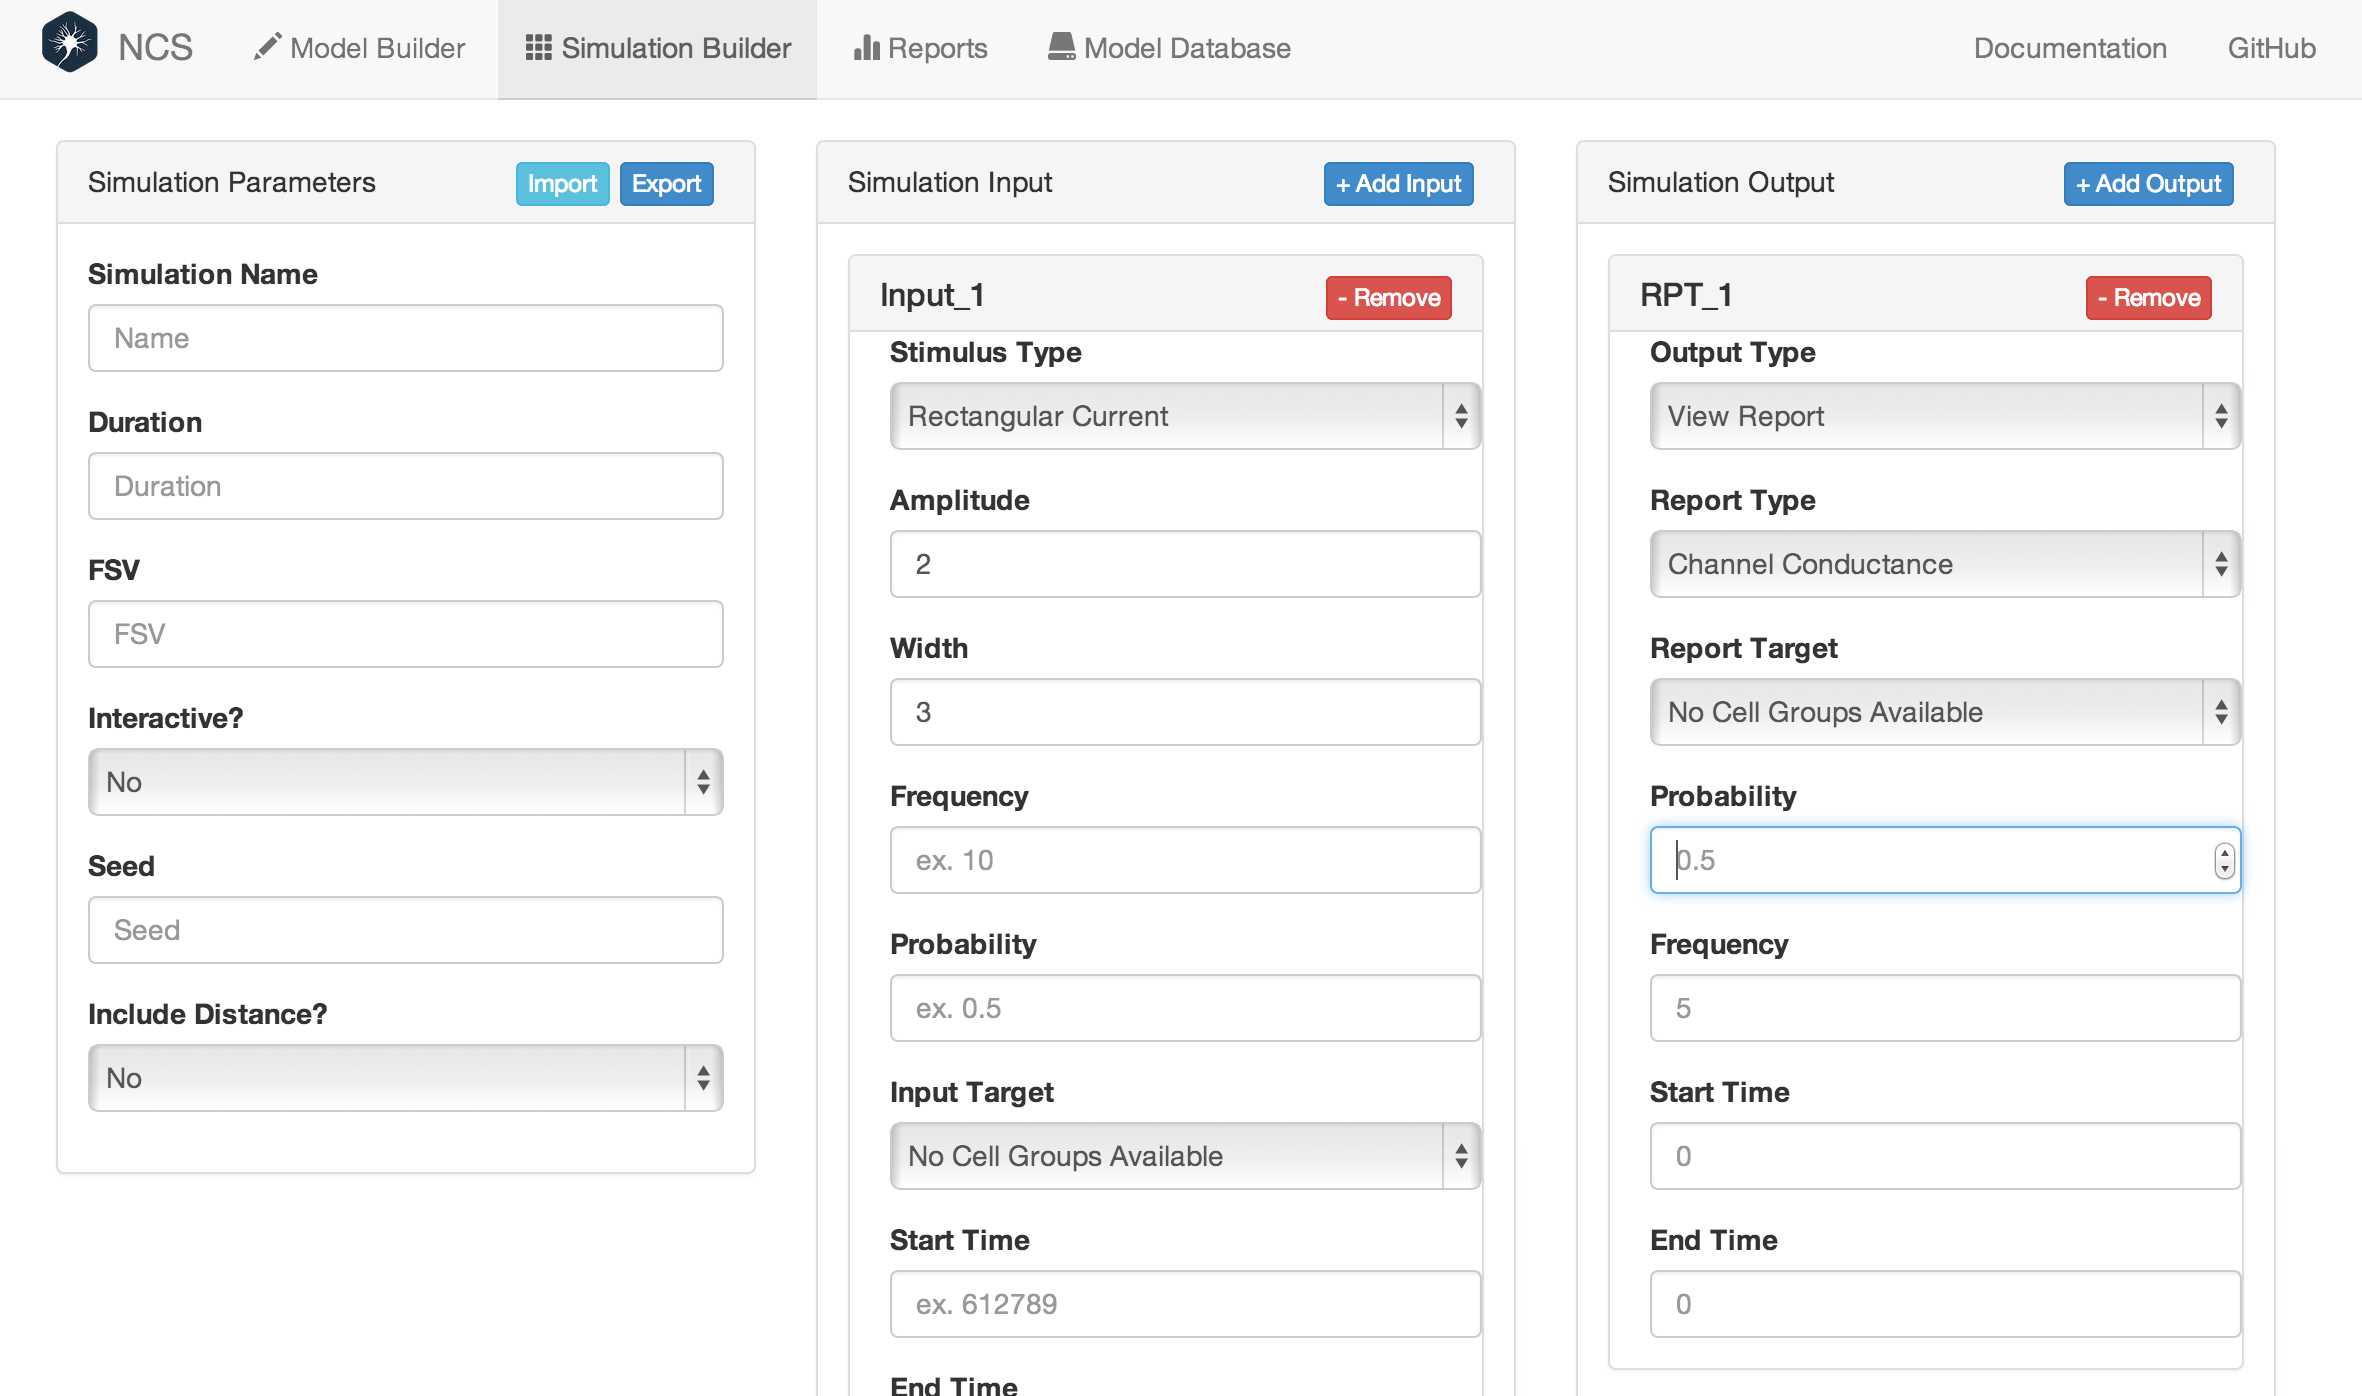
\includegraphics[height=\textheight,width=5in,keepaspectratio]{figures/sim_builder.png}
\caption[Sim Builder]{The sim builder provides the functionality for adding reports and stimuli to the simulation. The leftmost panel changes global simulation parameters, the middle panel controls stimuli, and the rightmost panel controls reports.\label{fig:sim_builder}}
\end{center}
\end{figure}

To view the results of a simulation, the user navigates to the report tab which is shown in Figure \ref{fig:reports}. The reports tab has the ability to view graphs of simulation data. This data can come from either a static report after the simulation has finished, or be streamed from NCS-Daemon and the simulator to the browser via a WebSocket interface. This feature gives researchers the ability to view simulation data in real-time. Graphs can be built from the data and exported to an SVG (vector) format for inclusion in high quality publications and posters. An example of one of these graphs is shown in Figure \ref{fig:report_graph}.

\begin{figure}
\begin{center}
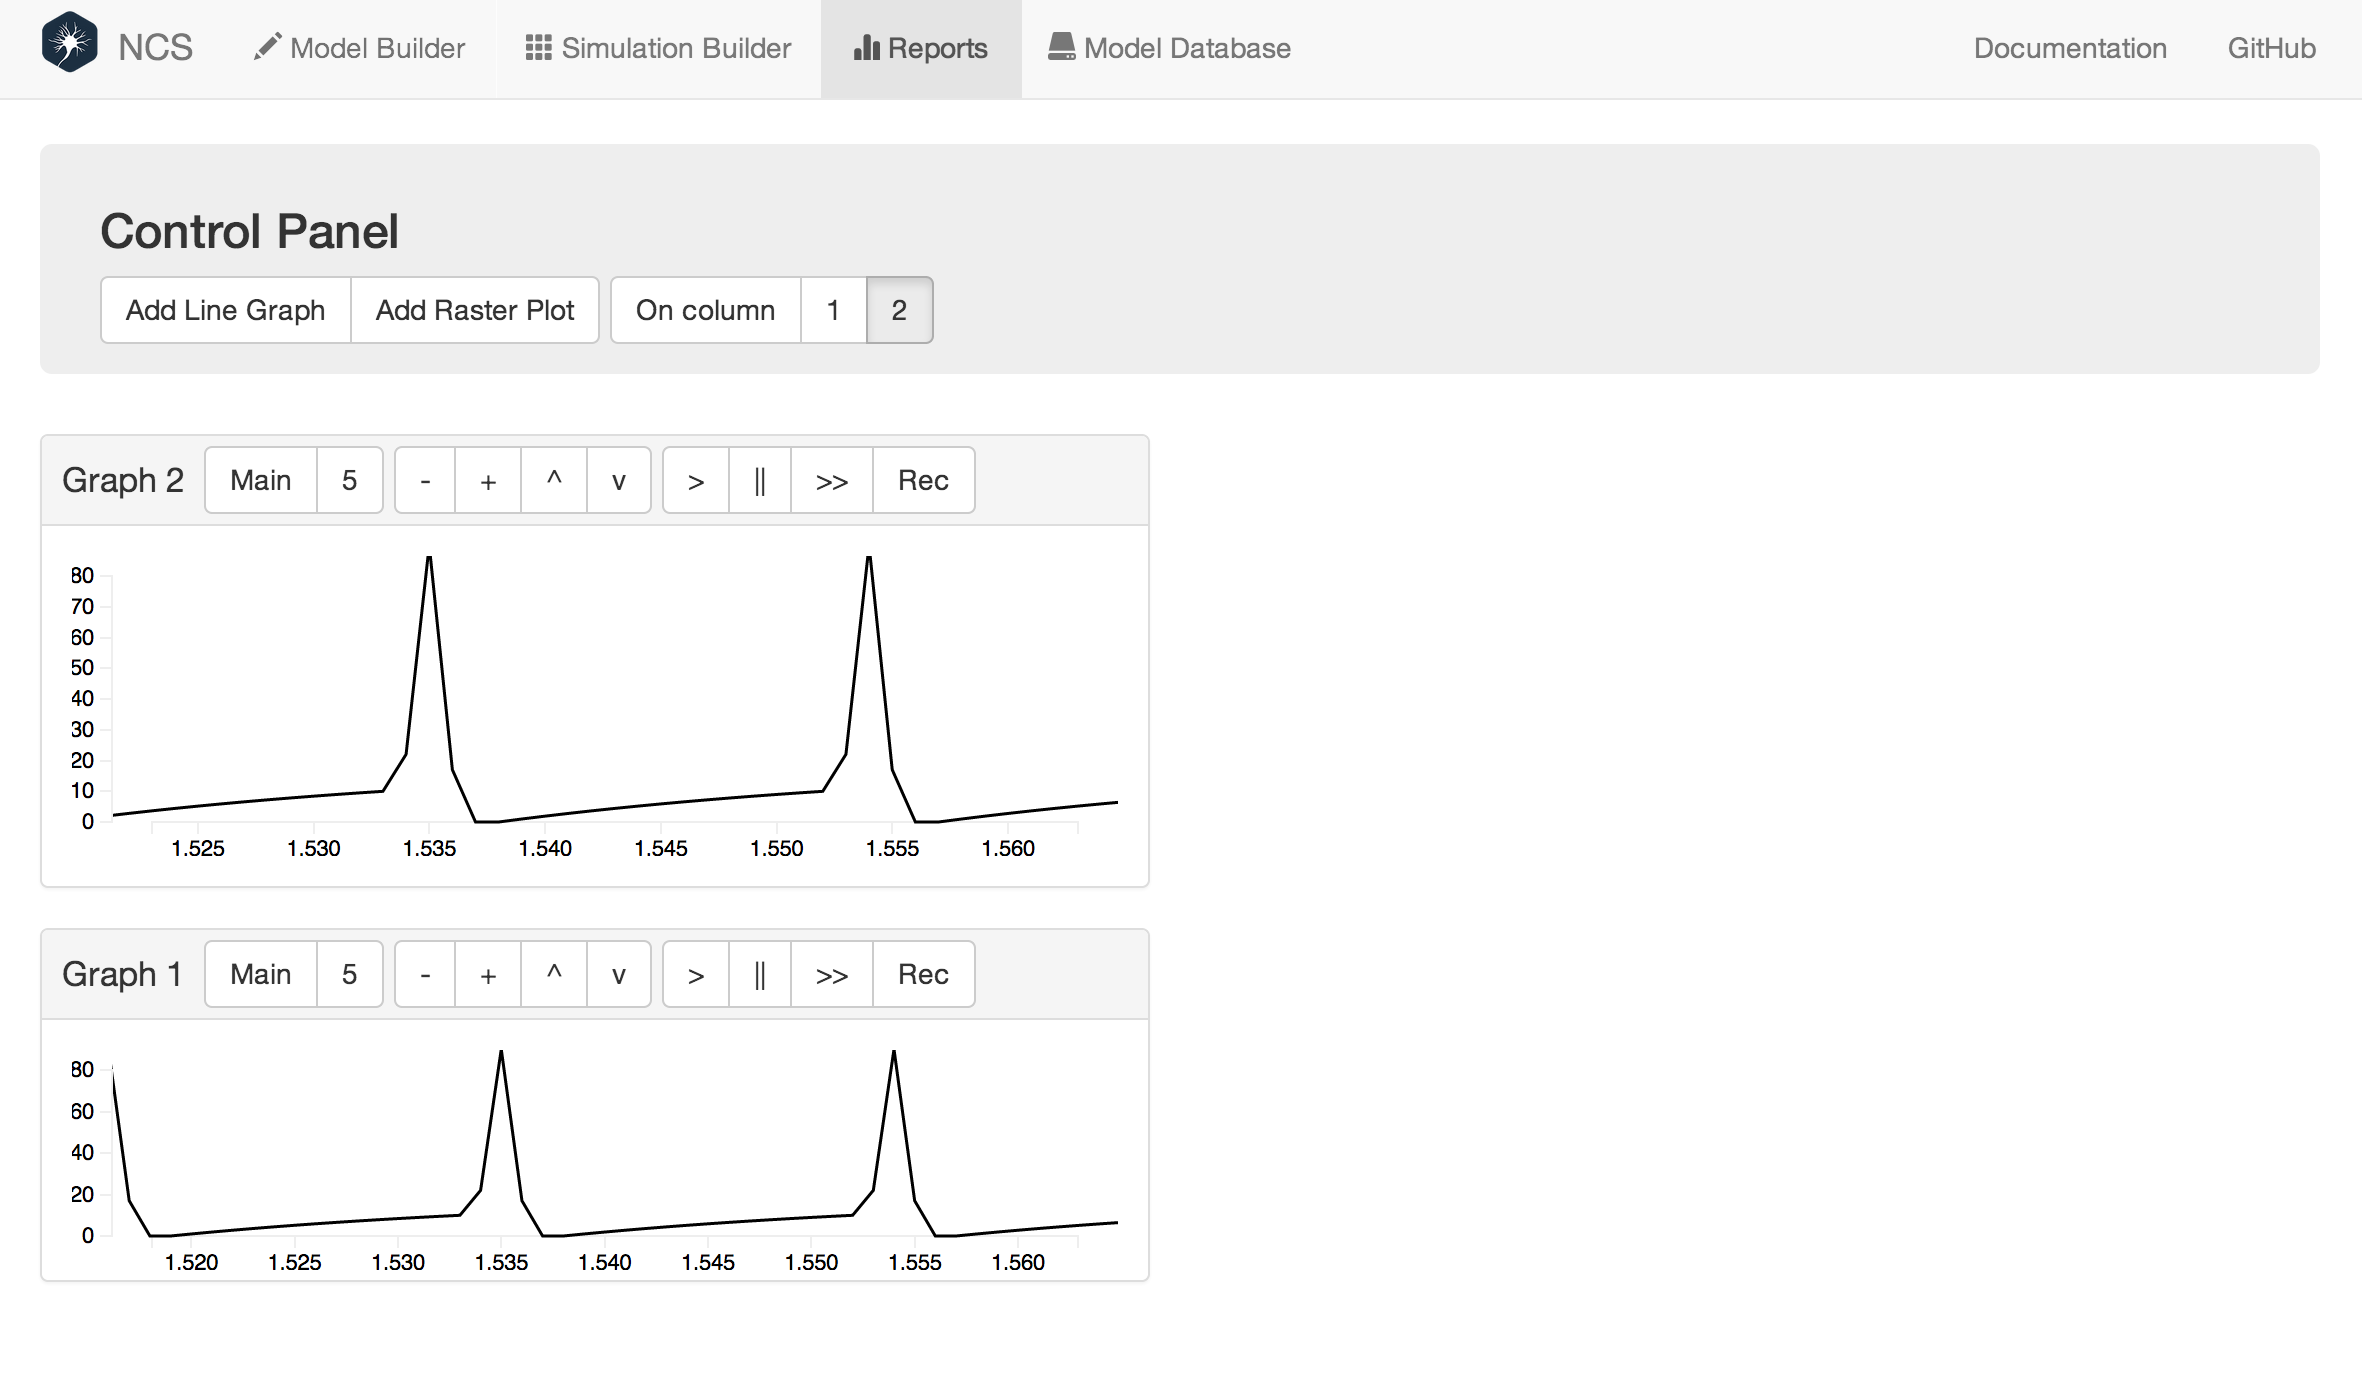
\includegraphics[height=\textheight,width=5in,keepaspectratio]{figures/reports.png}
\caption[Reports]{The reports tab allows users to view static and realtime data about a simulation. The graphs can be saved as high-quality SVG images for presentations or reports.\label{fig:reports}}
\end{center}
\end{figure}

\begin{figure}
\begin{center}
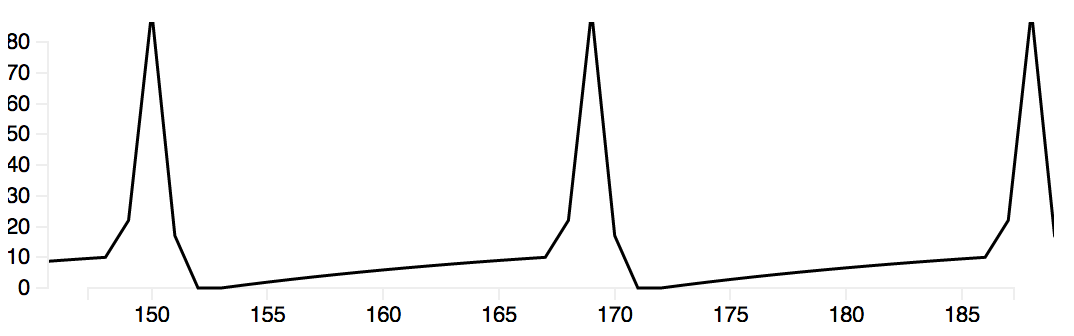
\includegraphics[height=\textheight,width=5in,keepaspectratio]{figures/report_graph.png}
\caption[Report Graph]{The reports generated in the reports tab can be exported as high-quality images for use in publications or in presentations.\label{fig:report_graph}}
\end{center}
\end{figure}

The robot simulation tab is still heavily in development. It allows simulation output to control the actions of a virtual robot in a 3D world and allow the observations of the robot on its environment to become inputs to the simulator. The simulator could be used to demonstrate the decision making ability of a brain model with the actions of the robot in the virtual environment, such as navigating a maze or performing actions when recognizing colors or patterns.







